Consider the following activity diagram:



\begin{centering}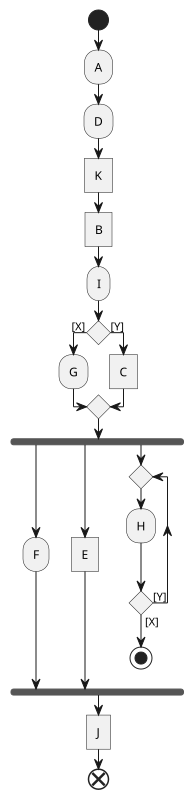
\includegraphics[min width=0.4\textwidth=0.6\textwidth,min height=0.4\textwidth=0.6\textwidth,keepaspectratio,max width=0.9\textwidth,max height=0.9\textwidth]{67/Diagram.pdf}\end{centering}

State the names of all action nodes, the names of all object nodes, and the count of each other kind of element for the given activity diagram.

To do this, enter your answer as in the following example:\begin{verbatim}MatchAdSolution {actionNodeNames = ["A","B"], objectNodeNames = ["C","D"], countOfDecisionNodes = 2, countOfMergeNodes = 2, countOfForks = 0, countOfJoins = 0, countOfInitialNodes = 1, countOfActivityFinalNodes = 1, countOfFlowFinalNodes = 0}\end{verbatim}

